%%%%%%%%%%%%%%%%%%%%%%%%%%%%%%%%%%%%%%%%%
% AOS Thesis and Dissertation Template
%   in LaTeX
% Version 0.3 (05/06/16)
%
% AOS version:
% Ethan Nelson
% http://github.com/ethan-nelson/AOS_thesis_template
%
% Original authors:
% Steven Gunn 
% http://users.ecs.soton.ac.uk/srg/softwaretools/document/templates/
% and
% Sunil Patel
% http://www.sunilpatel.co.uk/thesis-template/
% Later customization by www.latextemplates.com.
%
% License:
% CC BY-NC-SA 3.0 (http://creativecommons.org/licenses/by-nc-sa/3.0/)
%
% Note:
% Make sure to edit document variables in the Config.tex file
%
%%%%%%%%%%%%%%%%%%%%%%%%%%%%%%%%%%%%%%%%%

%----------------------------------------------------------------------------------------
%	PACKAGES AND OTHER DOCUMENT CONFIGURATIONS
%----------------------------------------------------------------------------------------

\documentclass[12pt,letterpaper,oneside]{Thesis}
\usepackage{titlesec}
\usepackage{multirow}
\usepackage{hhline}
\usepackage{afterpage}
\usepackage{pdflscape}
\usepackage[comma, sort&compress]{natbib}

\titlespacing{\section}{0pt}{0pt}{-0.35cm}
\titlespacing{\subsection}{0pt}{0pt}{-0.35cm}

\usetikzlibrary{shapes.arrows,fadings}

\hypersetup{colorlinks=false}
\title{\ttitle}


\begin{document}

\frontmatter 

\setstretch{1.5} % Line spacing of 1.3

\newcommand{\HRule}{\rule{\linewidth}{0.5mm}}

%----------------------------------------------------------------------------------------
%	DOCUMENT VARIABLES
%	Fill in the lines below to customize your thesis.
%----------------------------------------------------------------------------------------
\authors{Buckingham U. \textsc{Badger}} % Your name; use \textsc{Last Name} for your last name

\thesistitle{On the Importance of an Atmosphere} % Your thesis title

\degree{Master of Science} % Your degree level

\committeenameone{Dr. Verner E. \textsc{Suomi}} % Your committee chair
\committeeroleone{Committee Chair}
\committeenametwo{Dr. Reid A. \textsc{Bryson}} % Another faculty member
\committeeroletwo{Faculty Member}
\committeenamethree{Dr. Louis W. \textsc{Uccellini}} % Yet another faculty member
\committeerolethree{Faculty Member}

\graduationmonth{December}
\graduationyear{2014}
%----------------------------------------------------------------------------------------     % Import customizations (e.g. author name)

% PDF meta-data
\hypersetup{pdftitle={\ttitle}}
\hypersetup{pdfauthor=\authornames}

\makeatletter
\renewcommand\chapter{\if@openright\cleardoublepage\else\clearpage\fi
                    \thispagestyle{fancy}
                    \global\@topnum\z@
                    \@afterindentfalse
                    \secdef\@chapter\@schapter}
\makeatother
\titlespacing*{\chapter}{0cm}{-2\topskip}{0pt}[0pt]
%\makeatletter
%\def\@makechapterhead#1{%
%  \vspace*{-50\p@}%
%  {\parindent \z@ \raggedright \normalfont
%    \ifnum \c@secnumdepth >\m@ne
%      \if@mainmatter
%        \huge\bfseries \@chapapp\space \thechapter
%        \par\nobreak
%        \vskip 20\p@
%      \fi
%    \fi
%    \interlinepenalty\@M
%    \Huge \bfseries #1\par\nobreak
%    \vskip 40\p@
%  }}
%\def\@makeschapterhead#1{%
%  \vspace*{-50\p@}%
%  {\parindent \z@ \raggedright
%    \normalfont
%    \interlinepenalty\@M
%    \Huge \bfseries  #1\par\nobreak
%    \vskip 40\p@
%  }}
%\makeatother

%----------------------------------------------------------------------------------------
%	TITLE PAGE
%----------------------------------------------------------------------------------------

\begin{titlepage}
\begin{center}

\HRule \\[0.4cm]
\setstretch{3}
{\huge \bfseries \ttitle}\\[0.4cm]
\setstretch{1.8}
\HRule \\[1.5cm]

\begin{center} \large
\authornames 
\end{center}
 
\large A thesis submitted in partial fulfillment of \\ the requirements for the degree of\\[1cm]
\degreename \\
(\subjectname) \\[1cm]
 at the\\
\textsc{\univname}\\
{\large \graduationmonth \ \graduationyear}\\[4cm]
%\includegraphics{Logo} % University/department logo 
 
\vfill
\end{center}

\end{titlepage}

%----------------------------------------------------------------------------------------
%	DECLARATION PAGE - Don't edit
%----------------------------------------------------------------------------------------

\Declaration{}

%----------------------------------------------------------------------------------------
%	PAGE HEADER DEFINITION - Don't edit
%        These are currently formatted to match the Graduate School's specifications
%----------------------------------------------------------------------------------------

\pagestyle{fancy}
\fancyhead{}
\renewcommand{\headrulewidth}{0pt}
\rhead{\thepage}

%----------------------------------------------------------------------------------------
%	ABSTRACT PAGE
%----------------------------------------------------------------------------------------

\setstretch{2}
\addtotoc{Abstract}
\addtocounter{page}{-1}

\abstract{

The atmosphere is a crucial part of everyday life by providing biological matter to respirate. Other planets in our solar system are characterized by a lack of atmosphere and thus remain unsuitable for life. Modeling a planet with no atmosphere resolves many of the issues plagued by modellers, especially pertaining to the issue of magnitudes of scales.

}

%----------------------------------------------------------------------------------------
%	QUOTATION PAGE
%----------------------------------------------------------------------------------------

\clearpage

\quotable{

\textit{``Thanks to my solid academic training, today I can write hundreds of words on virtually any topic without possessing a shred of information, which is how I got a good job in journalism."}

\begin{flushright}
Dave Barry
\end{flushright}

}

%----------------------------------------------------------------------------------------
%	DEDICATION
%----------------------------------------------------------------------------------------

\clearpage

\setstretch{1.3}
\dedicatory{

This work is dedicated to the love of my life, Python.

}

%----------------------------------------------------------------------------------------
%	ACKNOWLEDGEMENTS
%----------------------------------------------------------------------------------------

\clearpage

\setstretch{1.5}

\acknowledgements{

There are many people that made this possible. 

First, my advisor advised me very well.

Second, my colleagues and flatmates were very collegial.

Finally, my mom and dad have been parental to me.

Thanks to the data repository for providing data used in this thesis.

Acknowledgement is also made to the Department of Research for support under grants \#1, 5, and 290. 

}

%----------------------------------------------------------------------------------------
%	LIST OF CONTENTS/FIGURES/TABLES PAGES - Don't edit
%----------------------------------------------------------------------------------------

\clearpage

\begingroup
\tableofcontents % Write out the Table of Contents

\listoffigures % Write out the List of Figures

\listoftables % Write out the List of Tables
\endgroup

%----------------------------------------------------------------------------------------
%	ABBREVIATIONS
%----------------------------------------------------------------------------------------

\clearpage

\listofabbreviations{ll}
{

%\textbf{Acronym} & \textbf{W}hat (it) \textbf{S}tands \textbf{F}or \\
\textbf{CPR} & \textbf{C}loud \textbf{P}rofiling \textbf{R}adar (aboard CloudSat) \\
\textbf{MJO} & \textbf{M}adden-\textbf{J}ulian Oscillation \\
\textbf{TRMM} & \textbf{T}ropical \textbf{R}ainfall \textbf{M}easuring \textbf{M}ission 

}

%----------------------------------------------------------------------------------------
%	PHYSICAL CONSTANTS/OTHER DEFINITIONS
%----------------------------------------------------------------------------------------

\clearpage

\listofconstants{lrcl}
{

Speed of Light & $c$ & $=$ & $2.997\ 924\ 58\times10^{8}\ \mbox{ms}^{-\mbox{s}}$ (exact)\\
% Constant Name & Symbol & = & Constant Value (with units) \\

}

%----------------------------------------------------------------------------------------
%	SYMBOLS
%----------------------------------------------------------------------------------------

\clearpage

\listofnomenclature{lll}
{

$a$ & distance & m \\
$P$ & power & W (Js$^{-1}$) \\
% Symbol & Name & Unit \\

& & \\ % Gap to separate the Roman symbols from the Greek

$\omega$ & angular frequency & rads$^{-1}$ \\
% Symbol & Name & Unit \\

}

%----------------------------------------------------------------------------------------
%	THESIS CONTENT: CHAPTERS - Don't edit unless you have 10 or more chapters
%----------------------------------------------------------------------------------------

\mainmatter
\setstretch{2.0}

\IfFileExists{./Chapters/Chapter1.tex}{% Chapter 1

\chapter{Introduction} % Chapter title

\label{Chapter1} % Change X to a consecutive number; for referencing this chapter elsewhere, use \ref{ChapterX}

%----------------------------------------------------------------------------------------
%	Chapter text below
%----------------------------------------------------------------------------------------

\section{Preface}\label{section:preface}
This is \sref{section:preface} that provides all of the information about my background. Be sure to check out \ssref{subsection:postscript} as well for more information. Please find \fref{atrain} for more information.

\subsection{Preface Postscript}\label{subsection:postscript}
Sometimes it is necessary to provide information about the background in segments.

\subsection{Postpostscript}

\begin{figure}[h]
\centering
	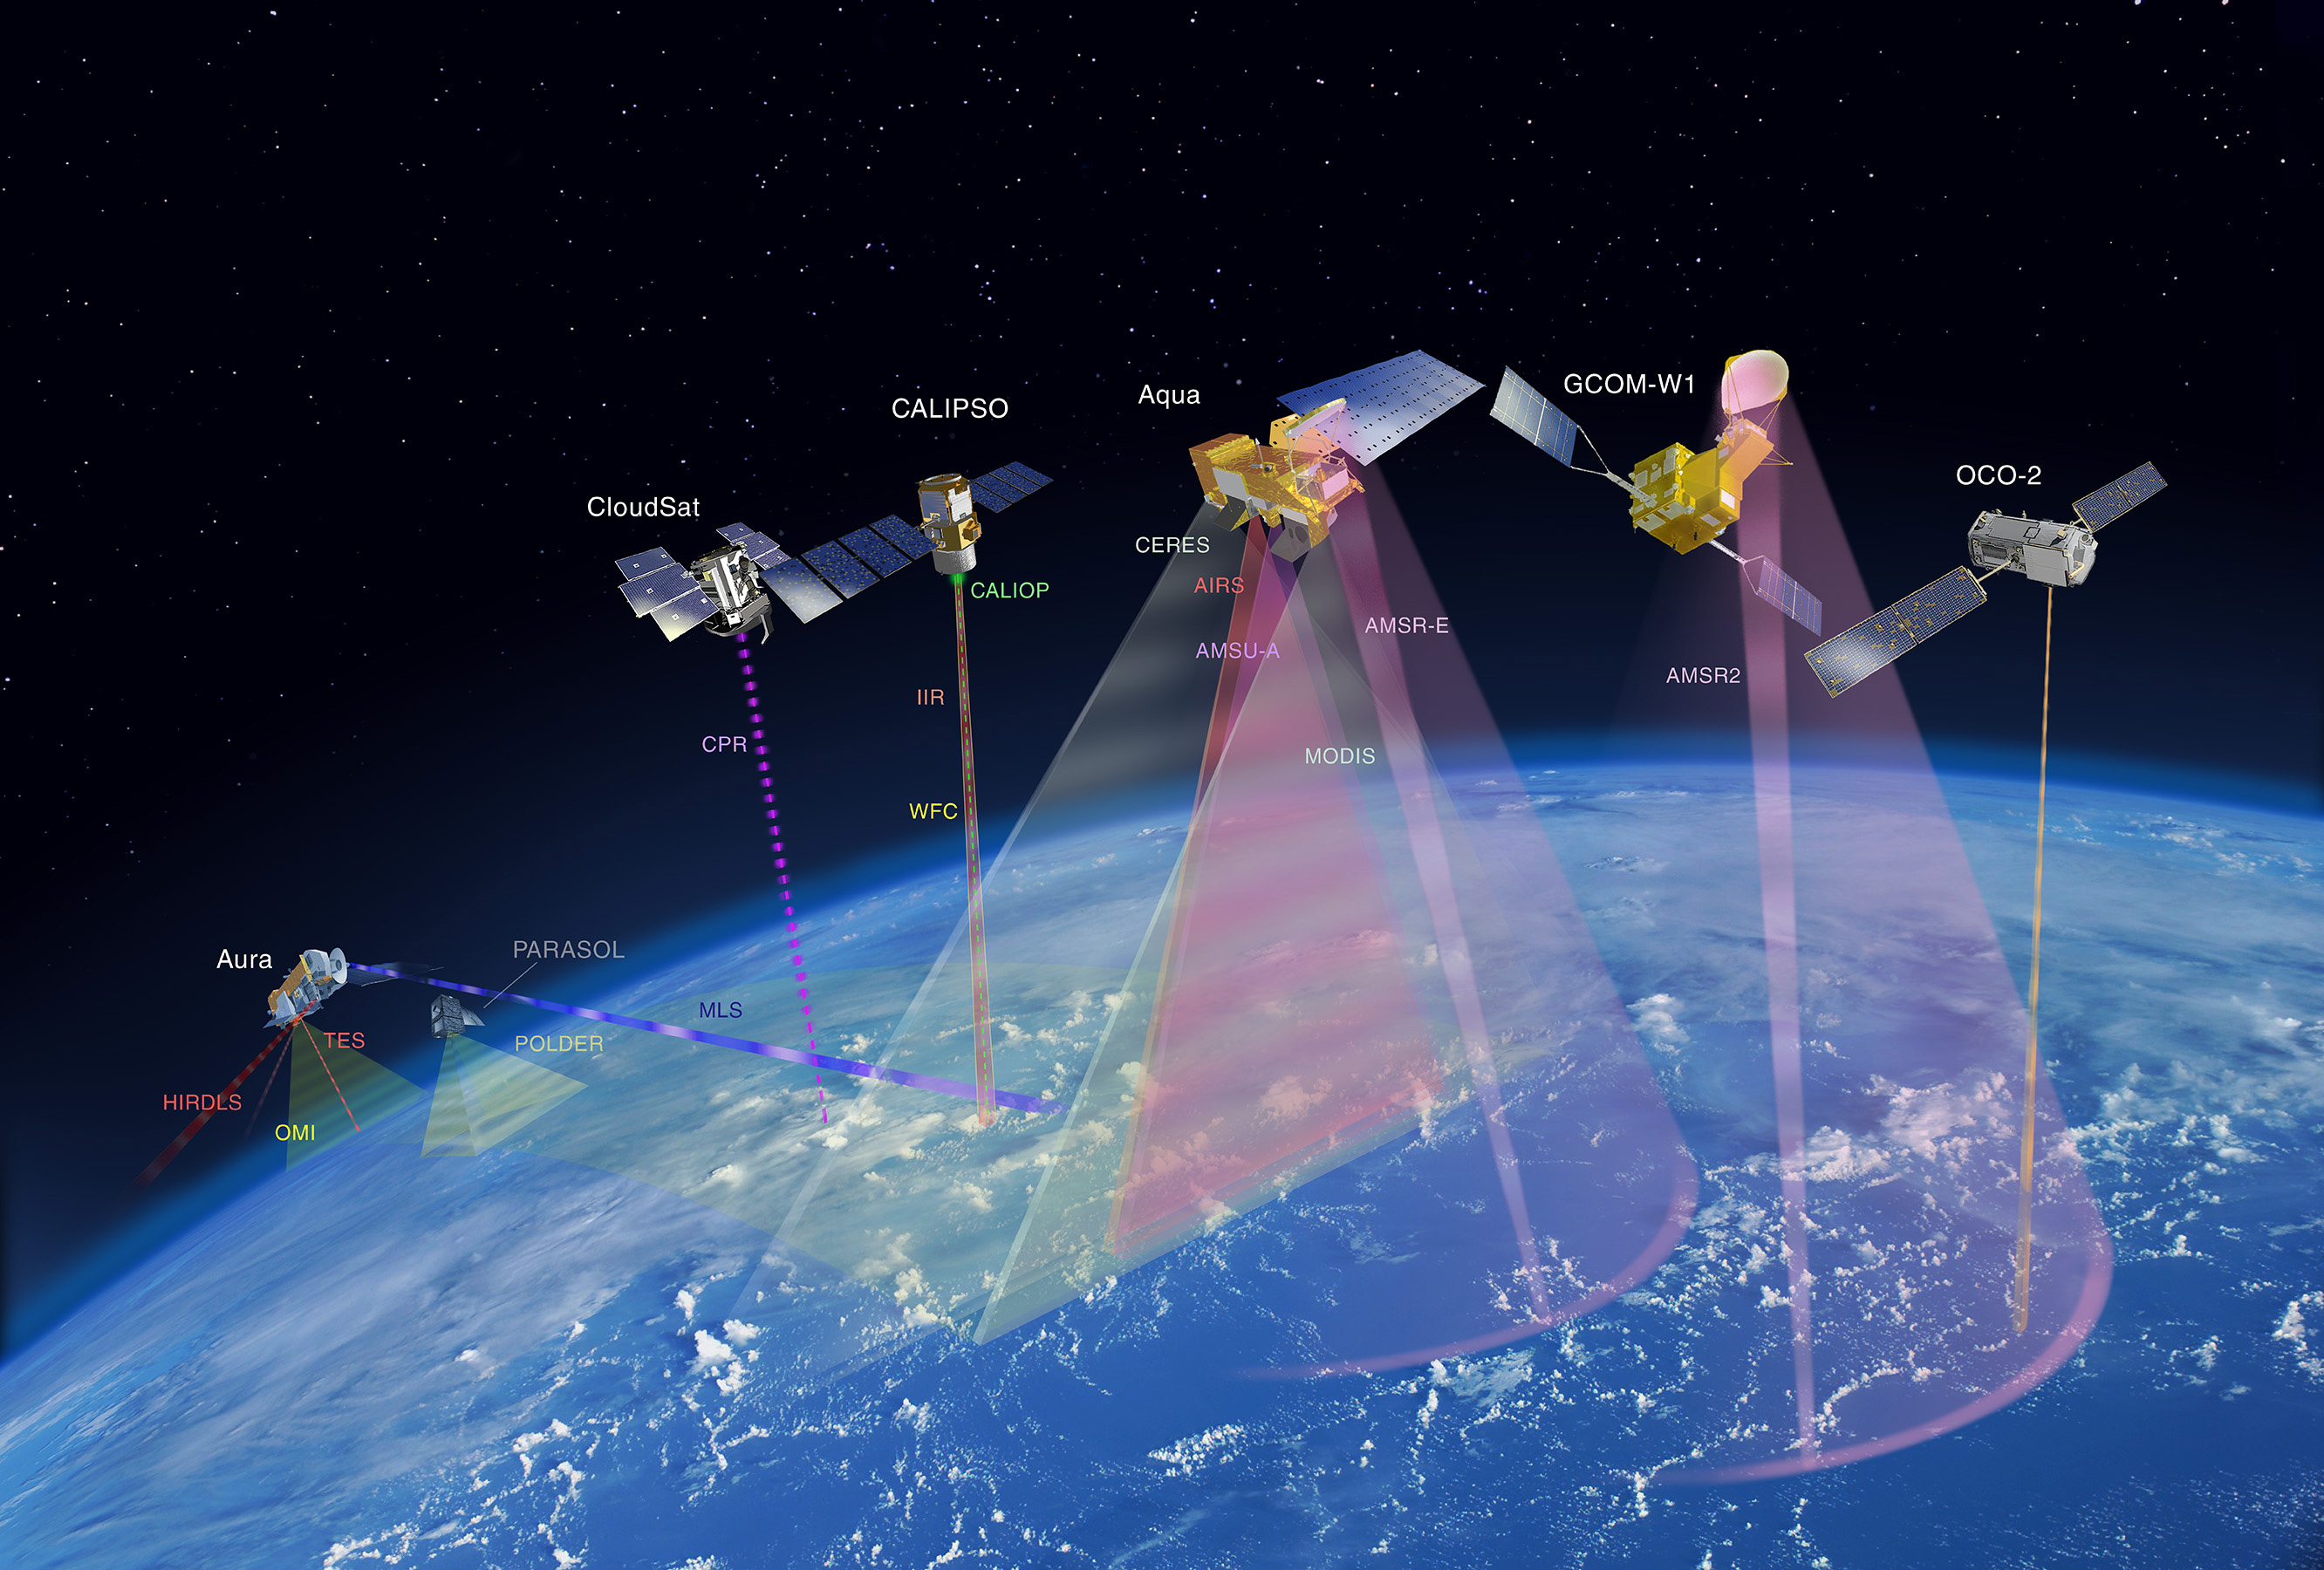
\includegraphics[width=0.6\linewidth]{Figures/atrain.jpeg}
	\rule{35em}{0.5pt}
	\caption[Afternoon Constellation illustration]{An illustration of the Afternoon Constellation (A-Train) satellite mission of NASA with the satellites' respective instruments. CloudSat is second from the left. Illustration courtesy of NASA.}\label{atrain}
\end{figure}

Other areas of interest.

Blah

Blah

\begin{table}[h]
    \centering
    \begin{tabular}{l|l|l}
    ~          & Header 1 & Header 2 \\ \hline \hline
    Category 1 & Data 11  & Data 21  \\ \hline
    Category 2 & Data 12  & Data 22  \\
    \end{tabular}
    \rule{35em}{0.5pt}
    \caption[Short title here.]{We have some data here.}
\end{table}

\begin{itemize}
\item In case you don't know \LaTeX{}
\end{itemize}

\begin{enumerate}
\item \citet{Tanelli2008} is relevant to the material at hand \cite{Tanelli2008}.
\end{enumerate}}{}
\IfFileExists{./Chapters/Chapter2.tex}{\input{Chapters/Chapter2}}{}
\IfFileExists{./Chapters/Chapter3.tex}{\input{Chapters/Chapter3}}{}
\IfFileExists{./Chapters/Chapter4.tex}{\input{Chapters/Chapter4}}{}
\IfFileExists{./Chapters/Chapter5.tex}{\input{Chapters/Chapter5}}{}
\IfFileExists{./Chapters/Chapter6.tex}{\input{Chapters/Chapter6}}{}
\IfFileExists{./Chapters/Chapter7.tex}{\input{Chapters/Chapter7}}{}
\IfFileExists{./Chapters/Chapter8.tex}{\input{Chapters/Chapter8}}{}
\IfFileExists{./Chapters/Chapter9.tex}{\input{Chapters/Chapter9}}{}

%----------------------------------------------------------------------------------------
%	THESIS CONTENT: APPENDICES - Don't edit unless you have 10 or more appendices
%----------------------------------------------------------------------------------------

\IfFileExists{./Appendices/AppendixA.tex}{

\addtocontents{toc}{\vspace{2em}}

\appendix

\IfFileExists{./Appendices/AppendixA.tex}{% Appendix A

\chapter{Appendix of Information} % Main appendix title

\label{AppendixA} % For referencing this appendix elsewhere, use \ref{AppendixA}

\lhead{Appendix A. \emph{Appendix of Information}} % This is for the header on each page - perhaps a shortened title

Here's information about stuff that isn't necessary in the regular chapters, but should be in the appendix.}{}
\IfFileExists{./Appendices/AppendixB.tex}{\input{Appendices/AppendixB}}{}
\IfFileExists{./Appendices/AppendixC.tex}{\input{Appendices/AppendixC}}{}
\IfFileExists{./Appendices/AppendixD.tex}{\input{Appendices/AppendixD}}{}
\IfFileExists{./Appendices/AppendixE.tex}{\input{Appendices/AppendixE}}{}
\IfFileExists{./Appendices/AppendixF.tex}{\input{Appendices/AppendixF}}{}
\IfFileExists{./Appendices/AppendixG.tex}{\input{Appendices/AppendixG}}{}
\IfFileExists{./Appendices/AppendixH.tex}{\input{Appendices/AppendixH}}{}
\IfFileExists{./Appendices/AppendixI.tex}{\input{Appendices/AppendixI}}{}

\addtocontents{toc}{\vspace{2em}}

\backmatter

}{}

%----------------------------------------------------------------------------------------
%	BIBLIOGRAPHY
%----------------------------------------------------------------------------------------

\IfFileExists{Thesis.bib}{

\clearpage
\label{References}

\bibliographystyle{ametsoc}

\bibliography{Thesis}

}{}
%----------------------------------------------------------------------------------------
%
%----------------------------------------------------------------------------------------
\end{document}  
